%!TEX TS-program = xelatex
\documentclass[]{friggeri-cv}
\usepackage{afterpage}
\usepackage{fontawesome}
\usepackage{hyperref}
\usepackage{color}
\usepackage{xcolor}
\usepackage{multirow}
\usepackage{array}
\usepackage{tabu}
\hypersetup{
    pdftitle={},
    pdfauthor={},
    pdfsubject={},
    pdfkeywords={},
    colorlinks=false,       % no link border color
    allbordercolors=white   % white border color for all
}
\RequirePackage{xcolor}
\definecolor{darkred}{HTML}{9F033B}

\begin{document}
\header{Danielle}{O'Sullivan}
      {\-\hspace{1.5cm} Application Developer | Accenture Technology}
      
% Fake text to add separator      
\fcolorbox{white}{black}{\parbox{\dimexpr\textwidth-2\fboxsep-2\fboxrule}{%
.....
}}

% In the aside, each new line forces a line break
\begin{aside}
  \section{}
    {
\includegraphics[scale=0.1]{img/circledp.png}}
    ~
	\section{Address}
		73 Stanton House
		Coxhill Way
		Aylesbury
		HP21 8FQ
		~
  \section{Mobile \& Email}
    07935 117 254
    \href{mailto:danielle.osullivan@accenture.com}{\textbf{danielle.osullivan@}\\accenture.com}
    ~
  \section{Social}
    \href{https://www.linkedin.com/in/danielleosullivan}{
\includegraphics[scale=0.015]{img/linkedin.jpg} danielleosullivan}
    \href{https://github.com/danielleos}{
\includegraphics[scale=0.025]{img/github.png} danielleos}
		%\href{http://danielleosullivan.com}{\textbf{danielleosullivan.com} % Not ready yet
    ~
  \section{Programming}
    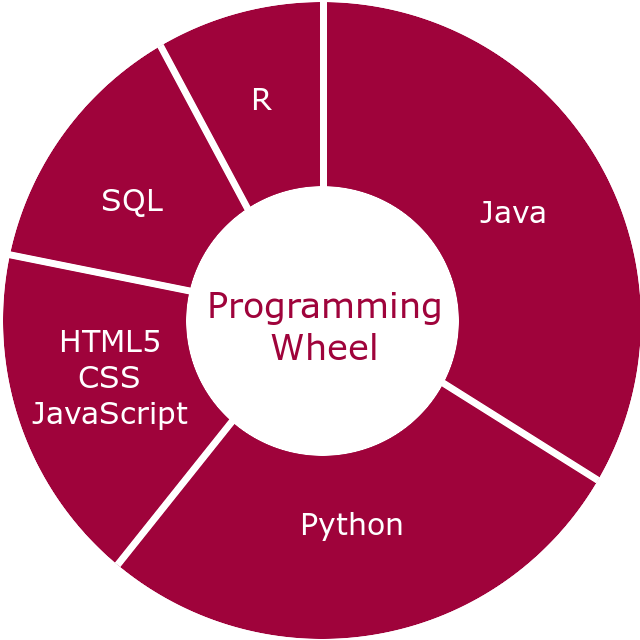
\includegraphics[scale=0.15]{img/programmingwheel.png}
    ~
  \section{Languages}
    \textbf{English}
\includegraphics[scale=0.40]{img/5stars.png}
    \textbf{Spanish}
\includegraphics[scale=0.40]{img/3stars.png}
    \textbf{Japanese}
\includegraphics[scale=0.40]{img/2stars.png}
    ~
    \section{Sport}
        \textbf{Dodgeball}:
        Played as part of the 1st Team in the WDPL in 2016-17.
        \textbf{Taekwon-Do}:
        Blue Belt
        5 gold, 4 silver, 3 bronze at national level in 2014-16.
        \textbf{Gymnastics}:
        Placed 7th at national level in 2007.
    ~
\end{aside}

\section{Profile}
      Danielle joined Accenture in September 2017 immediately after graduating from the University of Warwick with a BSc (Hons) Data Science degree. Most recently she has completed external Java SE8 Training with QA aiming to complete the Oracle Certified Associate exam in January 2018.\\
      
      She has experience in building Java applications at university including a virtual robot that navigates through mazes; a social media platform replica called 'Witter'; and a 'battle tank' bot using artificial intelligence theory and the RoboCode API.\\
      
      Some extra-curricular activities include participating in Google HashCode 2017; learning HTML, CSS, JavaScript \& Python using Codecademy and W3Schools; and producing high-quality documentation across the Software Development Life Cycle. At university she has represented her peers on the Data Science course as a member on the Statistics SSLC panel and was twice elected onto the executive committee for the Taekwon-Do club.

\section{Experience}
\begin{entrylist}
    \entry
    {09/17 - 11/17}
    {Application Development Associate}
    {Accenture}
    {Completed 3 weeks of Software Engineering virtual training using Pluralsight. Completed 1 week of External Java SE8 external classroom training with QA.\\}
    \entry
    {06/16 - 09/16}
    {IT Solutions Architect Intern}
    {Vodafone Group}
    {Presented a 1 hour ‘Knowledge Share’ on Big Data to the EIT Architecture Team. Produced documentation for End-to-End (E2E) product development. Completed IT Security Course.\\}
    \entry
    {02/12 - 09/14}
    {Founder \& Owner}
    {Orient UK}
    {Real-life application of Excel Solver. Demonstrated a high level of communication with both suppliers and customers.\\}
    %\entry
    %{07/11 - 08/13}
    %{Part-time Dental Nurse Assistant}
    %{Street Lane Dental Centre (SLDC)}
    %{Worked closely with dentists and dental nurses as either a pair or as a team of 3 to fulfill appointments.\\}
    %\entry
    %{09/09 - 07/11}
    %{Young Cub Scout Leader (Volunteer)}
    %{Holy Name of Jesus Parish}
    %{Successfully organised and ran weekly games with a group of average size of 20 scouts.\\}
\end{entrylist}

\section{Education}
\begin{entrylist}
  \entry % University
    {2014 - 2017}
    {BSc (Hons) in Data Science}
    {University of Warwick}
    {\emph{3rd Year:} Achieved a 1st in Social Informatics module. Completed an Individual Project in Predictive Analysis with Decision Trees (Python). Further modules: Machine Learning (Python), Neural Computing (Python), Computer Graphics (C++), Programming for Data Science (R) \& Topics in Data Science.\\\\
    \emph{2nd Year:} Achieved 2.1 grade in Software Engineering module (Java \& JavaScript). Further modules: Artificial Intelligence (Java), Database Systems (SQL \& Java), Mathematical \& Statistical methods.\\\\
    \emph{1st Year:} Achieved 2.1 grade in Linear Algebra \& Mathematical Programming I modules. Completed Japanese 1 course. Further modules: Design of Information Structures (Java), Introduction to Probability, Introduction to Java Programming.}
  \entry % A-Levels (Sixth Form)
    {2012 - 2014}
    {A-Levels}
    {St. Aidan's \& St. John Fisher Associated Sixth Form}
    {\emph{A2-level:} A*AA}
\end{entrylist}

\section{References}
\textbf{Sudhir Sarangapany}\\
Principal Enterprise IT Solutions Architect | Vodafone Group\\
\href{mailto:sudhir.sarangapany@vodafone.com}{\underline{sudhir.sarangapany@vodafone.com}}\\
07822 810 963

\end{document}
